\chapter{Begriffsexplikation}
% =================================================================
\thispagestyle{fancy}
\label{chap:begriffsexplikation}
% =================================================================
\section*{Isotropie}
\glqq Mit isotroper Strahlung ist in der Regel eine solche Strahlung gemeint, die in alle Richtungen des 3-dimensionalen Raumes gleichmäßig abgestrahlt wird.\grqq\;\cite{Isotropie}\\

\section*{Zentripetalkraft}
\begin{wrapfigure}{r}{0.4\textwidth}
\centering
\vspace{-2cm}
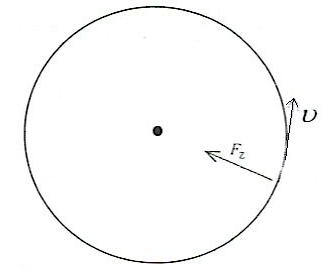
\includegraphics[scale=0.5]{Bilder/zentripetalkraft.png} 
\caption[Zentripetalkraft]{$F_{z}$ = Zentripetalkraft;\\ $v$ = Geschwindigkeit des Objektes \cite{Rudolph2017}}
\vspace{-2cm}
\label{fig:zentripetalkraft}
\end{wrapfigure}
\glqq Bei einer gleichförmigen Kreisbewegung wirkt auf den Körper stets eine Kraft, die immer zum Kreismittelpunkt zeigt. Diese Kraft wird als Zentripetalkraft bezeichnet.\grqq\;\cite{Rudolph2017}
\\[0.5cm]
In der Abbildung \ref{fig:zentripetalkraft} ist dies illustriert.\\

\section*{Aperiodizität}
Nicht periodisch oder auch das Fehlen einer periodischen Eigenschaft von einem Signal.\\

\section*{Ionisation}
\glqq Ionisation heißt jeder Vorgang, bei dem aus einem Atom oder Molekül ein oder mehrere Elektronen entfernt werden, so dass das Atom oder Molekül als positiv geladenes Ion zurückbleibt. Der Umkehrvorgang, bei dem ein Elektron von einem ionisierten Atom oder Molekül eingefangen wird, wird als Rekombination bezeichnet. Im weiteren Sinne könnte auch die Bildung negativer Ionen (durch Anlagerung eines zusätzlichen Elektrons an das neutrale Atom oder Molekül) als Ionisation bezeichnet werden.\grqq\; \cite{ionisation}\\

\section*{Stossionisation}
\glqq Bei der Stoßionisation in der ursprünglichen Wortbedeutung werden Elektronen durch einfallende, hinreichend schnelle Elektronen aus Atomen oder Molekülen „herausgeschlagen“ und diese dadurch ionisiert. Im weiteren Sinne kann man jede Ionisation so bezeichnen, die durch irgend einen Stoßvorgang (also beispielsweise beim photoelektrischen Effekt) erfolgt und nicht durch Wirkung eines elektrischen Feldes oder auf andere Weise.\grqq\; \cite{stossionisation}\\
\newpage
\section*{Photoionisation}
\glqq Unter Photoionisation (auch atomarer oder molekularer Photoeffekt) schließlich versteht man die Ionisierung von Atomen durch Bestrahlung mit Licht genügend hoher Frequenzen.\grqq\; \cite{photoionisation}\\